% !TeX root = ../main.tex
\section{Evaluación Experimental y Resultados}
\label{sec:evaluacion}

En esta sección se analiza cuantitativamente el comportamiento del sistema a lo largo del banco de pruebas experimental, respondiendo a las preguntas de investigación formuladas: el sobrecoste temporal de la capa de auditoría, el desacoplamiento de recursos físicos, la escalabilidad del consenso bizantino IBFT~2.0, la resiliencia empírica frente a ataques de adulteración y la previsibilidad del consumo de gas en la EVM. Con el objetivo de afianzar la solidez, robustez y reproducibilidad experimental, cada una de las cinco configuraciones experimentales ($E_1$ a $E_5$) fue evaluada a lo largo de 3 ejecuciones independientes completas de 30 rondas cada una, totalizando un corpus de 15 ejecuciones y 450 rondas federadas ($N_{\text{total}} = 450$).

\subsection{Convergencia del Modelo y Análisis de Pérdida}
La Figura~\ref{fig:convergencia} ilustra la evolución de la función de pérdida de entropía cruzada en el conjunto de validación durante las 30 iteraciones federadas.

\begin{figure}[H]
    \centering
    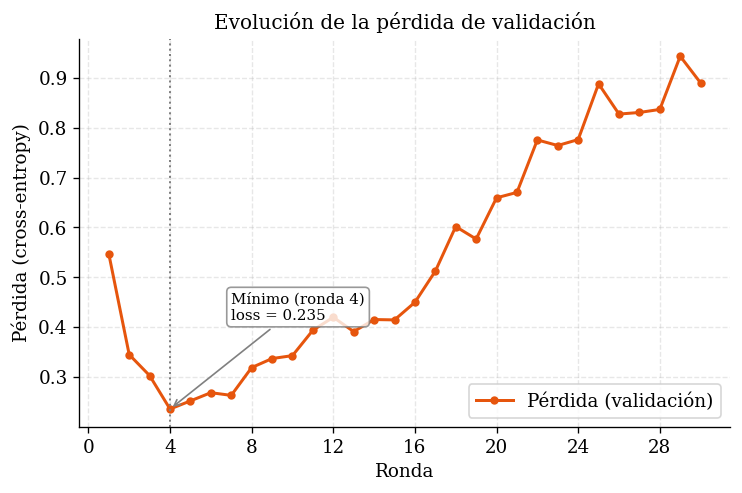
\includegraphics[width=\columnwidth]{figuras/convergencia_loss.png}
    \caption{Evolución de la pérdida de validación (\textit{cross-entropy}) a lo largo de las 30 rondas federadas.}
    \label{fig:convergencia}
\end{figure}

El modelo muestra un rápido aprendizaje inicial, alcanzando su mínimo de pérdida en la ronda 4 ($\mathcal{L} \approx 0{,}24$) con una precisión de clasificación que se estabiliza en el $97\%$. A partir de dicho punto, la pérdida experimenta un incremento gradual y sostenido hasta situarse en torno a $0{,}90$ hacia el final del ciclo. Este comportamiento representa un caso paradigmático de sobreajuste (\textit{overfitting}) provocado por el régimen de 90 épocas acumuladas (3 épocas locales $\times$ 30 rondas federadas) sobre un conjunto de entrenamiento acotado, donde la red incrementa excesivamente su confianza en predicciones.

El mínimo de pérdida en la ronda 4 sugiere que la incorporación de técnicas como la parada temprana (\textit{early stopping}) habría detenido el entrenamiento en ese instante, logrando una versión más ajustada del clasificador. Sin embargo, se mantuvieron de forma deliberada las 30 rondas predefinidas porque el objetivo central de esta investigación no es optimizar el modelo de IA ni perseguir su punto de máxima eficiencia, sino someter la infraestructura de aprendizaje federado a una carga constante para extraer métricas cuantitativas reproducibles (latencia por ronda, tiempo de confirmación y coste de gas). De este modo, la optimización fina del modelo se pospone como trabajo futuro.

Es fundamental enfatizar que \textbf{la curva de convergencia es estrictamente idéntica con o sin la presencia de Blockchain}. Dado que la capa de trazabilidad opera exclusivamente en la verificación e indexación criptográfica fuera de cadena y no interfiere en los tensores ni en los gradientes de FedAvg, la dinámica de entrenamiento se mantiene inalterada.

\subsection{Formalización Matemática de Métricas de Rendimiento}
Con el fin de aislar de forma unívoca la latencia impuesta por cada componente del sistema, el tiempo total por ronda en los nodos de borde ($T_{\text{client}}$) y en el servidor agregador ($T_{\text{server}}$) en la iteración $t$ se define analíticamente como:
\begin{align}
T_{\text{client}}^{(t)} &= t_{\text{verif\_desc}}^{(t)} + t_{\text{train}}^{(t)} + t_{\text{ipfs\_up}}^{(t)} + t_{\text{tx\_besu}}^{(t)} \label{eq:t_client} \\
T_{\text{server}}^{(t)} &= t_{\text{wait}}^{(t)} + t_{\text{verif\_asc}}^{(t)} + t_{\text{fedavg}}^{(t)} \nonumber \\
&\quad + t_{\text{ipfs\_global}}^{(t)} + t_{\text{block\_confirm}}^{(t)} \label{eq:t_server}
\end{align}
donde $t_{\text{verif\_desc}}$ representa la comprobación local contra el CID de Besu; $t_{\text{train}}$, el tiempo de cálculo de gradientes con PyTorch; $t_{\text{ipfs\_up}}$, la publicación binaria de pesos; $t_{\text{tx\_besu}}$, la emisión y confirmación de \texttt{registerClientModel}; $t_{\text{wait}}$, la ventana de recepción gRPC; $t_{\text{verif\_asc}}$, la validación en \texttt{getClientModel}; $t_{\text{fedavg}}$, la agregación matricial; y $t_{\text{block\_confirm}}$, la confirmación del bloque IBFT~2.0 tras invocar \texttt{updateModel}.

Es crucial destacar la complementariedad entre ambas perspectivas temporales:
\begin{itemize}
    \item \textbf{Tiempo de ciclo en el cliente ($T_{\text{client}}$, reportado en la Tabla~\ref{tab:tiempos_resumen}):} Cuantifica la duración de la computación y comunicación local en los nodos de borde (vehículos), desde que reciben el modelo global hasta que sellan su contribución en la Blockchain. Esta métrica gobierna la autonomía operativa de los clientes y mantiene la comparabilidad directa con los estudios previos~\cite{cloudlabaia_flblockchain}.
    \item \textbf{Tiempo de ronda extremo a extremo en el servidor ($T_{\text{server}}$, desglosado en la Tabla~\ref{tab:desglose_fases}):} Engloba la totalidad del ciclo orquestado por el agregador central, incorporando la sincronización gRPC de todos los clientes concurrentes y la inclusión en bloque del nuevo modelo global mediante \texttt{updateModel} ($\approx 2{,}8\text{--}5{,}1$~s adicionales por ronda).
\end{itemize}

Para medir el sobrecoste relativo ($\Delta_{\text{overhead}}$) entre una configuración con seguridad $E_{\text{BC}}$ y su respectiva línea base $E_{\text{base}}$, se emplea la mediana de las distribuciones:
\begin{equation}
\Delta_{\text{overhead}} = \frac{\text{Med}(T_{E_{\text{BC}}}) - \text{Med}(T_{E_{\text{base}}})}{\text{Med}(T_{E_{\text{base}}})} \times 100 \quad [\%] \label{eq:overhead}
\end{equation}

En cuanto al rigor metodológico del análisis estadístico, el diseño experimental considera como unidades muestrales independientes las \textbf{15 ejecuciones completas} ($N_{\text{runs}} = 3$ repeticiones independientes por cada una de las 5 configuraciones). Las 30 rondas federadas consecutivas de cada ejecución no se presentan como observaciones independientes idénticamente distribuidas (i.i.d.), ya que cada iteración $t+1$ depende intrínsecamente del estado paramétrico y las condiciones del sistema en la ronda $t$. Por consiguiente, las 450 rondas totales ($90$ por configuración) se emplean para el análisis descriptivo longitudinal y la visualización de trayectorias (Figura~\ref{fig:tiempo_todas}), mientras que la reproducibilidad inter-ejecución se cuantifica a través del Error Estándar ($SE$) entre las medias de las ejecuciones independientes ($SE = \sigma_{\text{runs}} / \sqrt{N_{\text{runs}}}$).

\subsection{Visión General del Rendimiento Temporal Consolidado}
La Tabla~\ref{tab:tiempos_resumen} sintetiza el tiempo de ciclo por ronda en los nodos de borde ($T_{\text{client}}$) a lo largo de las 15 ejecuciones independientes (3 por configuración, totalizando 90 rondas por entorno para análisis descriptivo continuo), reportando la mediana, media, desviación típica inter-ejecución ($\sigma_{\text{runs}}$) y error estándar ($SE = \sigma_{\text{runs}} / \sqrt{3}$). Asimismo, la Figura~\ref{fig:tiempo_todas} refleja la serie temporal continua a lo largo de las rondas.

\begin{table}[H]
\centering
\caption{Tiempo de ciclo por ronda en los nodos de borde ($T_{\text{client}}$) consolidado ($15$ ejecuciones independientes, $3$ por configuración, $30$ rondas/run). Los valores de $\sigma_{\text{runs}}$ y $SE$ cuantifican la dispersión y el error estándar entre las medias de las $3$ ejecuciones independientes ($SE = \sigma_{\text{runs}} / \sqrt{3}$).}
\label{tab:tiempos_resumen}
\resizebox{\columnwidth}{!}{%
\begin{tabular}{@{}cccccccc@{}}
\toprule
\textbf{Exp.} & \textbf{Máq.} & \textbf{Configuración} & \textbf{Runs} & \textbf{Mediana (s)} & \textbf{Media (s)} & \textbf{$\sigma_{\text{runs}}$ (s)} & \textbf{SE (s)} \\
\midrule
$E_1$ & 1 & 4 val · con BC & 3 & \textbf{85,42} & 97,09 & 20,01 & 11,55 \\
$E_2$ & 1 & Baseline sin BC & 3 & \textbf{75,70} & 76,45 & 1,65 & 0,95 \\
\midrule
$E_3$ & 2 & Baseline sin BC & 3 & \textbf{66,62} & 67,62 & 2,29 & 1,32 \\
$E_4$ & 2 & 4 val · con BC & 3 & \textbf{72,96} & 73,29 & 1,28 & 0,74 \\
$E_5$ & 2 & 7 val · con BC & 3 & \textbf{73,35} & 74,40 & 0,54 & 0,31 \\
\bottomrule
\end{tabular}%
}
\end{table}

\begin{figure}[H]
    \centering
    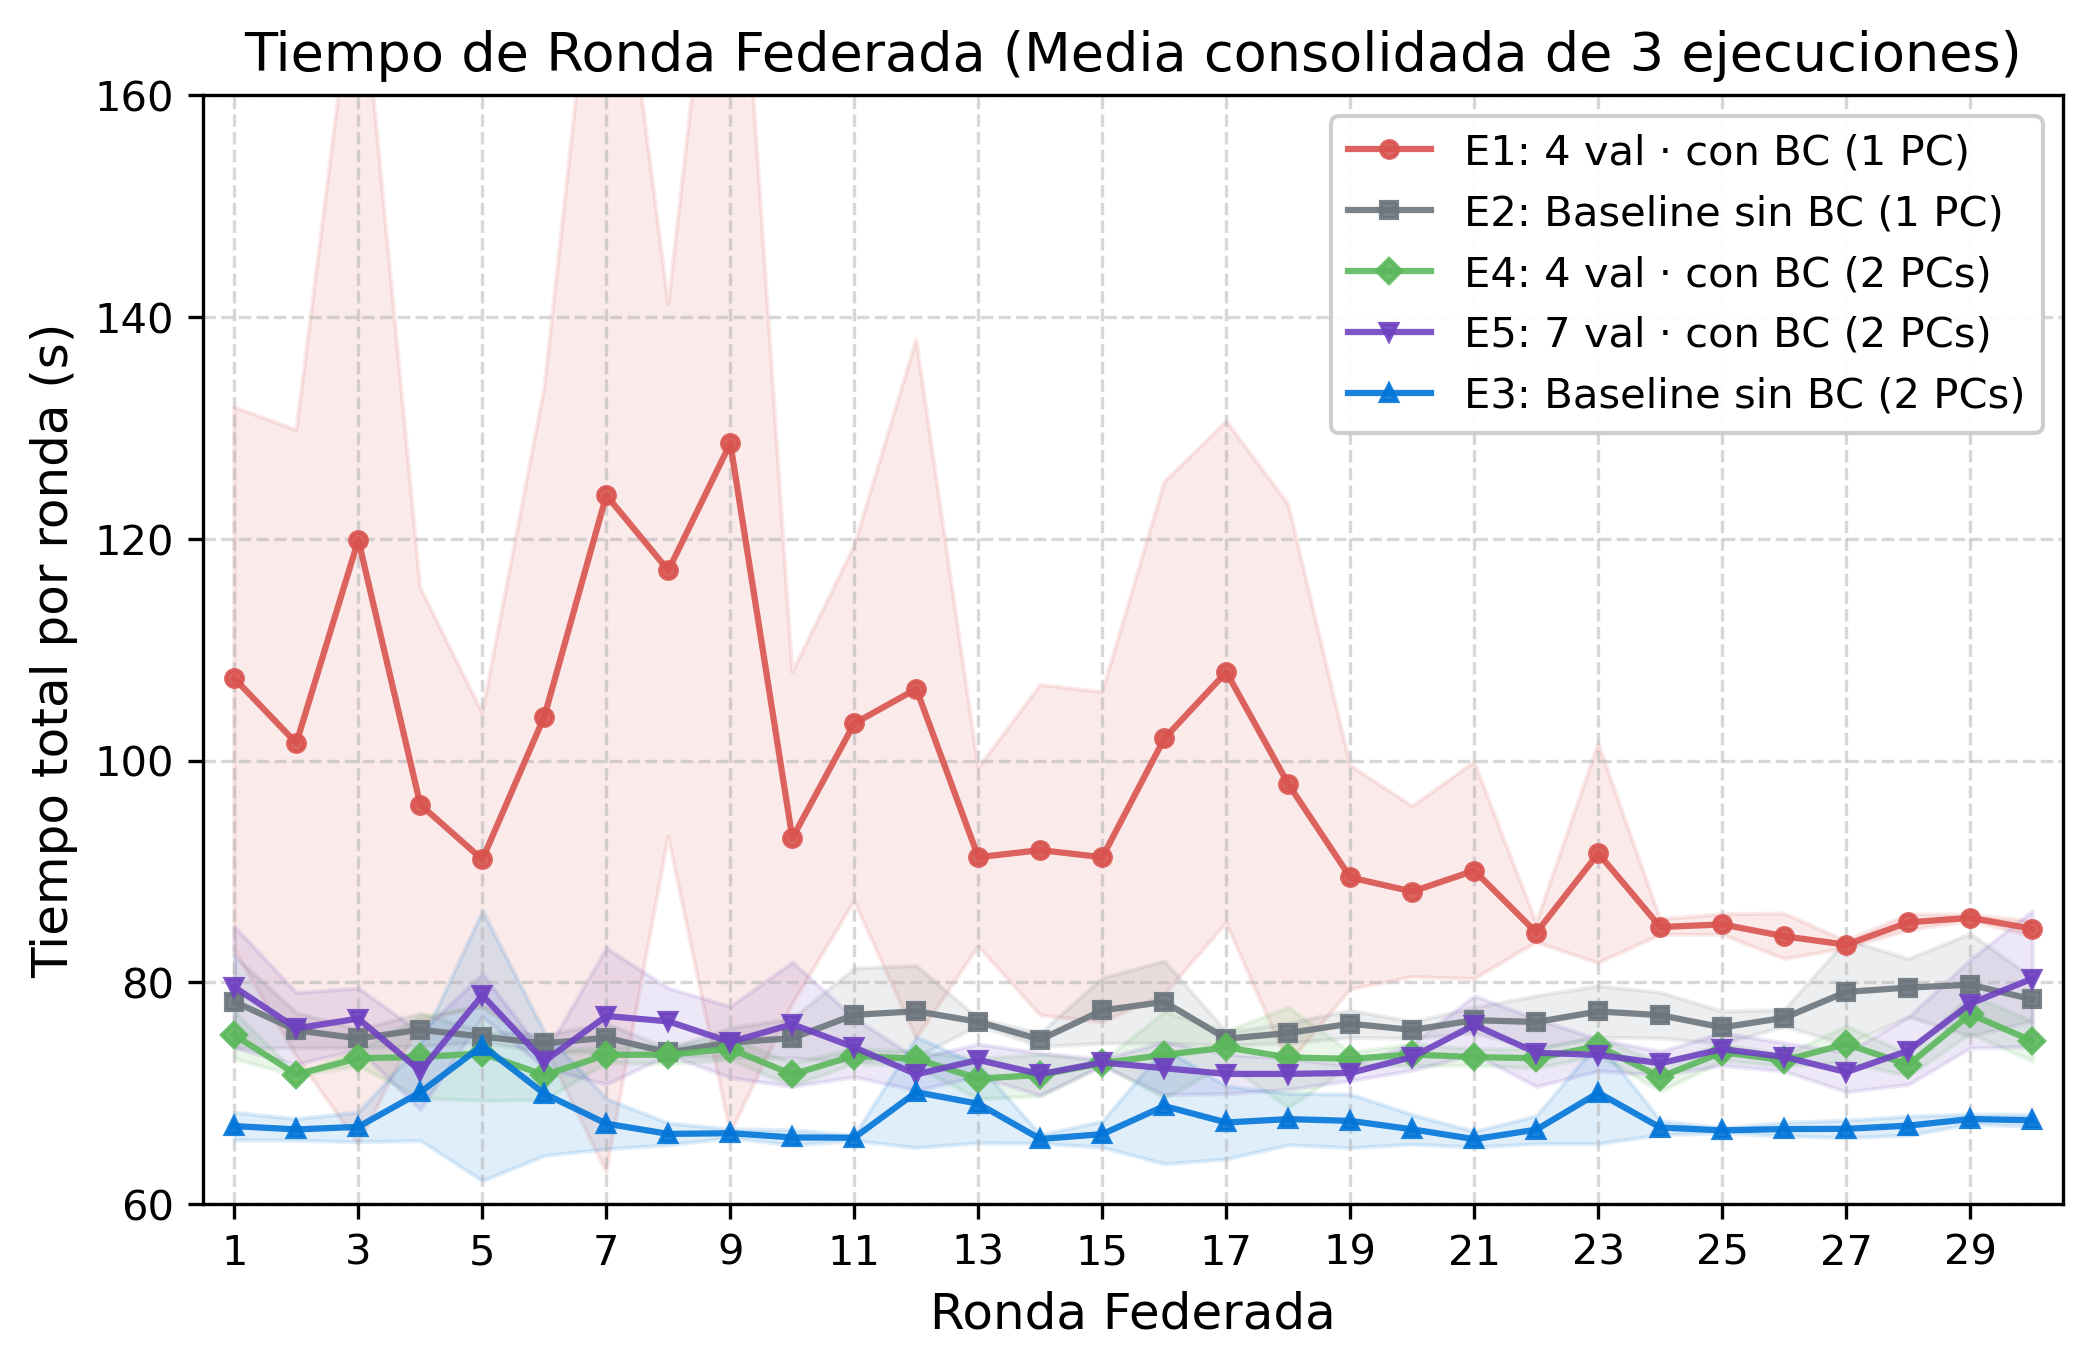
\includegraphics[width=\columnwidth]{figuras/tiempo_ronda_todas.png}
    \caption{Comparativa del tiempo de ciclo en clientes ($T_{\text{client}}$) a lo largo de las rondas en las cinco configuraciones experimentales.}
    \label{fig:tiempo_todas}
\end{figure}

El análisis multiejecución revela diferencias clave en la estabilidad de cada entorno. En la configuración local $E_1$, la dispersión inter-ejecución entre las medias de las tres repeticiones es de $\sigma_{\text{runs}} = 20{,}01$~s ($SE = 11{,}55$~s), registrando una dispersión longitudinal acumulada a lo largo de las 90 rondas de $\sigma_{\text{pool}} = 27{,}64$~s. Esta mayor variabilidad se debe a que, en la primera ejecución en monomáquina, los procesos de entrenamiento convolucional compitieron directamente en CPU y memoria con los ocho contenedores de Docker que soportaban los nodos de Besu y el daemon de IPFS. Por el contrario, en el entorno distribuido ($E_4$ y $E_5$), la variabilidad inter-ejecución se reduce drásticamente ($\sigma_{\text{runs}} \in [0{,}54, 1{,}28]$~s y $SE \le 0{,}74$~s; con dispersiones longitudinales contenidas en $\sigma_{\text{pool}} \le 3{,}92$~s), demostrando una gran estabilidad y reproducibilidad operativa. Por este motivo, se adopta la \textbf{mediana} como métrica central para aislar el comportamiento intrínseco del sistema frente a fluctuaciones externas.

\subsection{Sobrecoste Temporal Aislado de la Capa Blockchain}
Para cuantificar con exactitud el coste temporal impuesto por la serialización de tensores, la publicación en IPFS, la firma ECDSA y el consenso IBFT~2.0, se comparan las configuraciones equivalentes con y sin capa de seguridad (Figura~\ref{fig:coste_bc}):
\begin{itemize}
    \item \textbf{Escenario Monomáquina ($E_1$ vs. $E_2$)}: El tiempo mediano pasa de 75,70~s a 85,42~s, representando un sobrecoste de \textbf{+9,72~s (+12,8\%)}.
    \item \textbf{Escenario Distribuido ($E_3$ vs. $E_4$)}: El tiempo mediano se incrementa de 66,62~s a 72,96~s, lo que supone una sobrecarga de tan solo \textbf{+6,34~s (+9,5\%)}.
\end{itemize}

\begin{figure}[H]
    \centering
    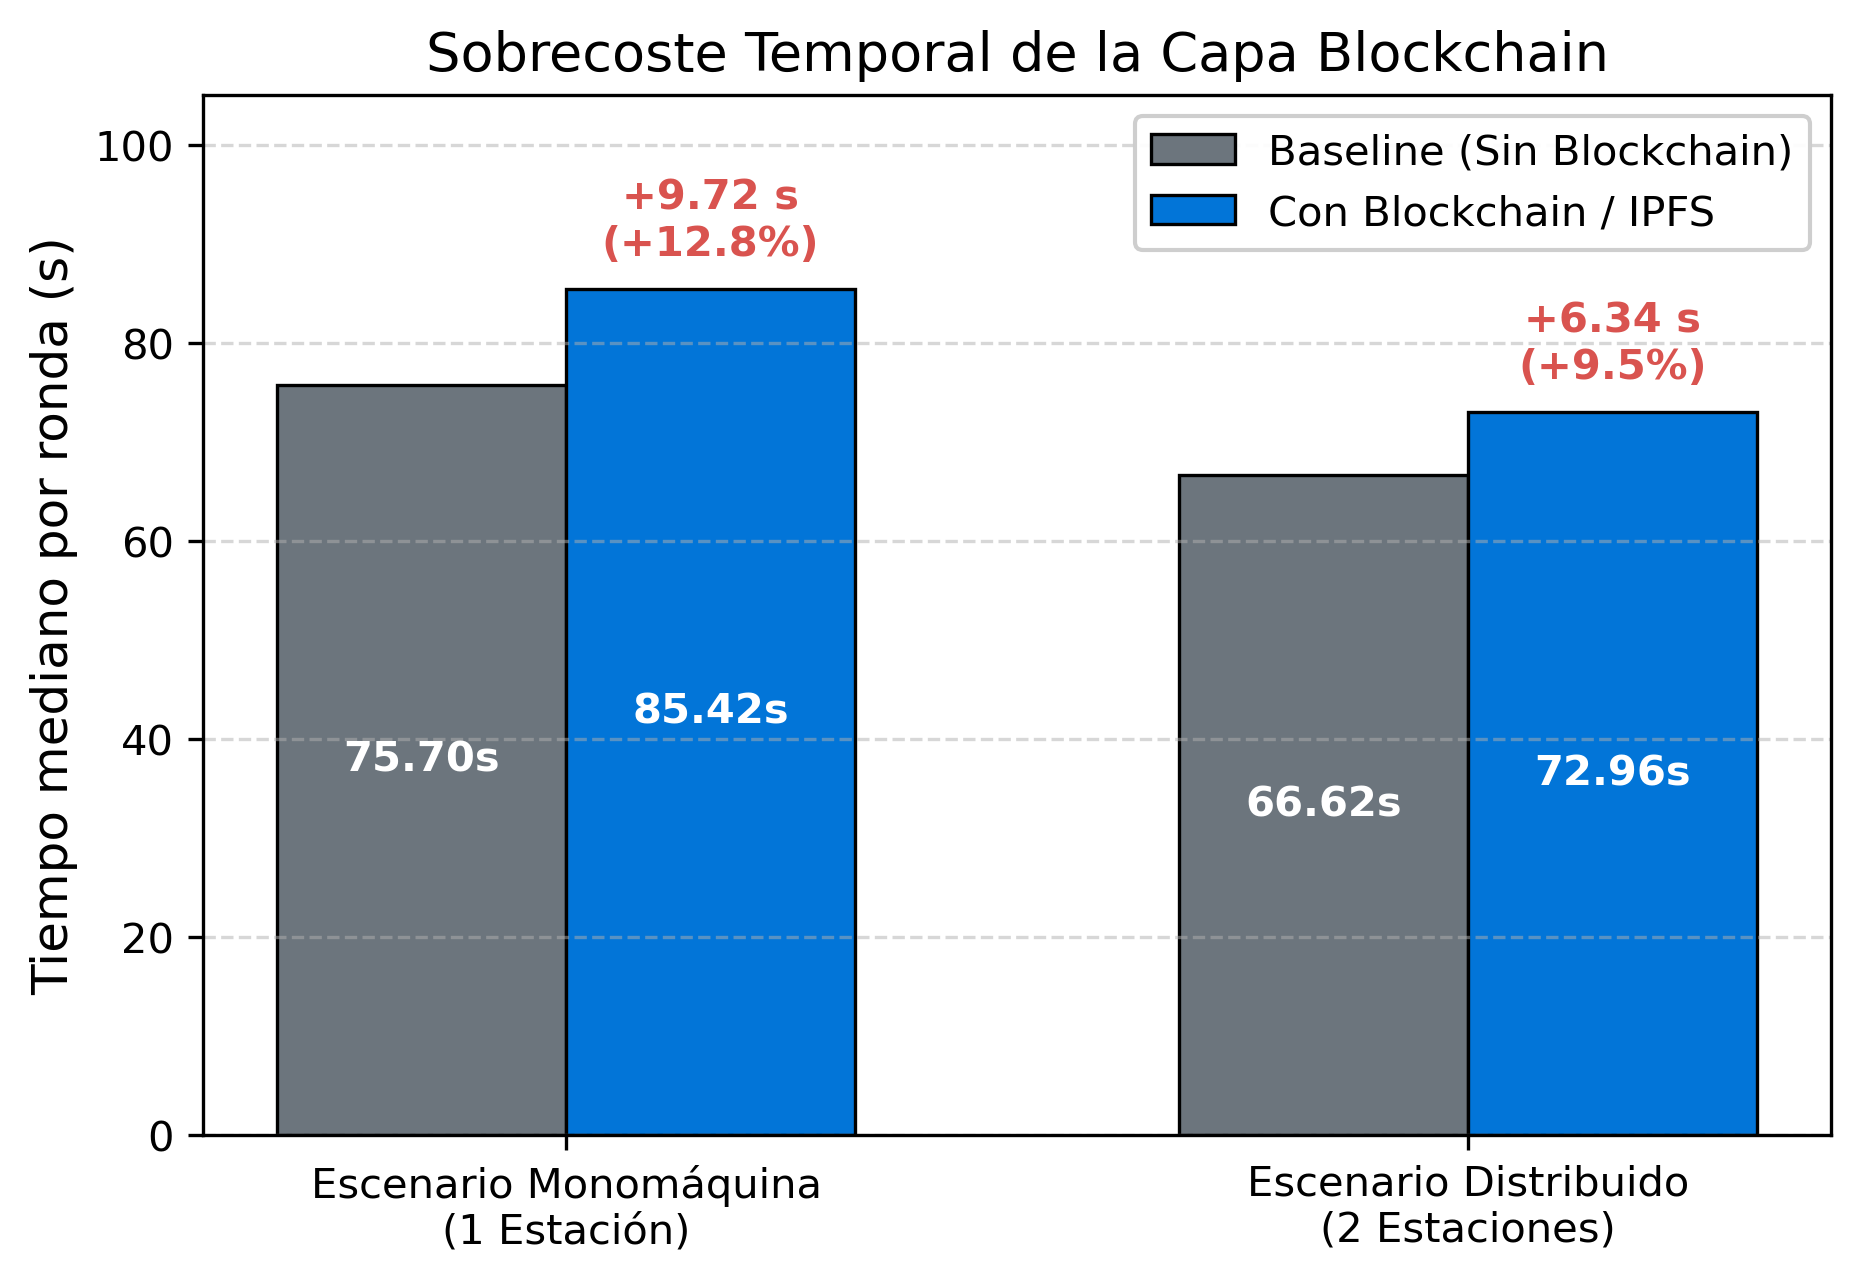
\includegraphics[width=\columnwidth]{figuras/coste_blockchain.png}
    \caption{Sobrecoste temporal inducido por la integración de la Blockchain en entornos local y distribuido.}
    \label{fig:coste_bc}
\end{figure}

Este hallazgo es de especial trascendencia para aplicaciones vehiculares y de borde: al desacoplar el entrenamiento de los clientes en una estación independiente, el impacto de la capa de auditoría e inmutabilidad se sitúa por debajo del 10\%. Una penalización de apenas 6 segundos por ronda resulta ampliamente asumible frente al beneficio de contar con un registro descentralizado inmutable y auditable.

\subsection{Efecto de la Distribución Física y Desglose por Fases}
La comparación entre la arquitectura monomáquina y distribuida demuestra que la separación física de roles optimiza el rendimiento global (Figura~\ref{fig:coste_dist}): el tiempo de ronda se reduce tanto en el baseline sin Blockchain (de 75,70~s a 66,62~s; un descenso de -12,0\%) como con Blockchain (de 85,42~s a 72,96~s; una reducción de -14,6\%).

\begin{figure}[H]
    \centering
    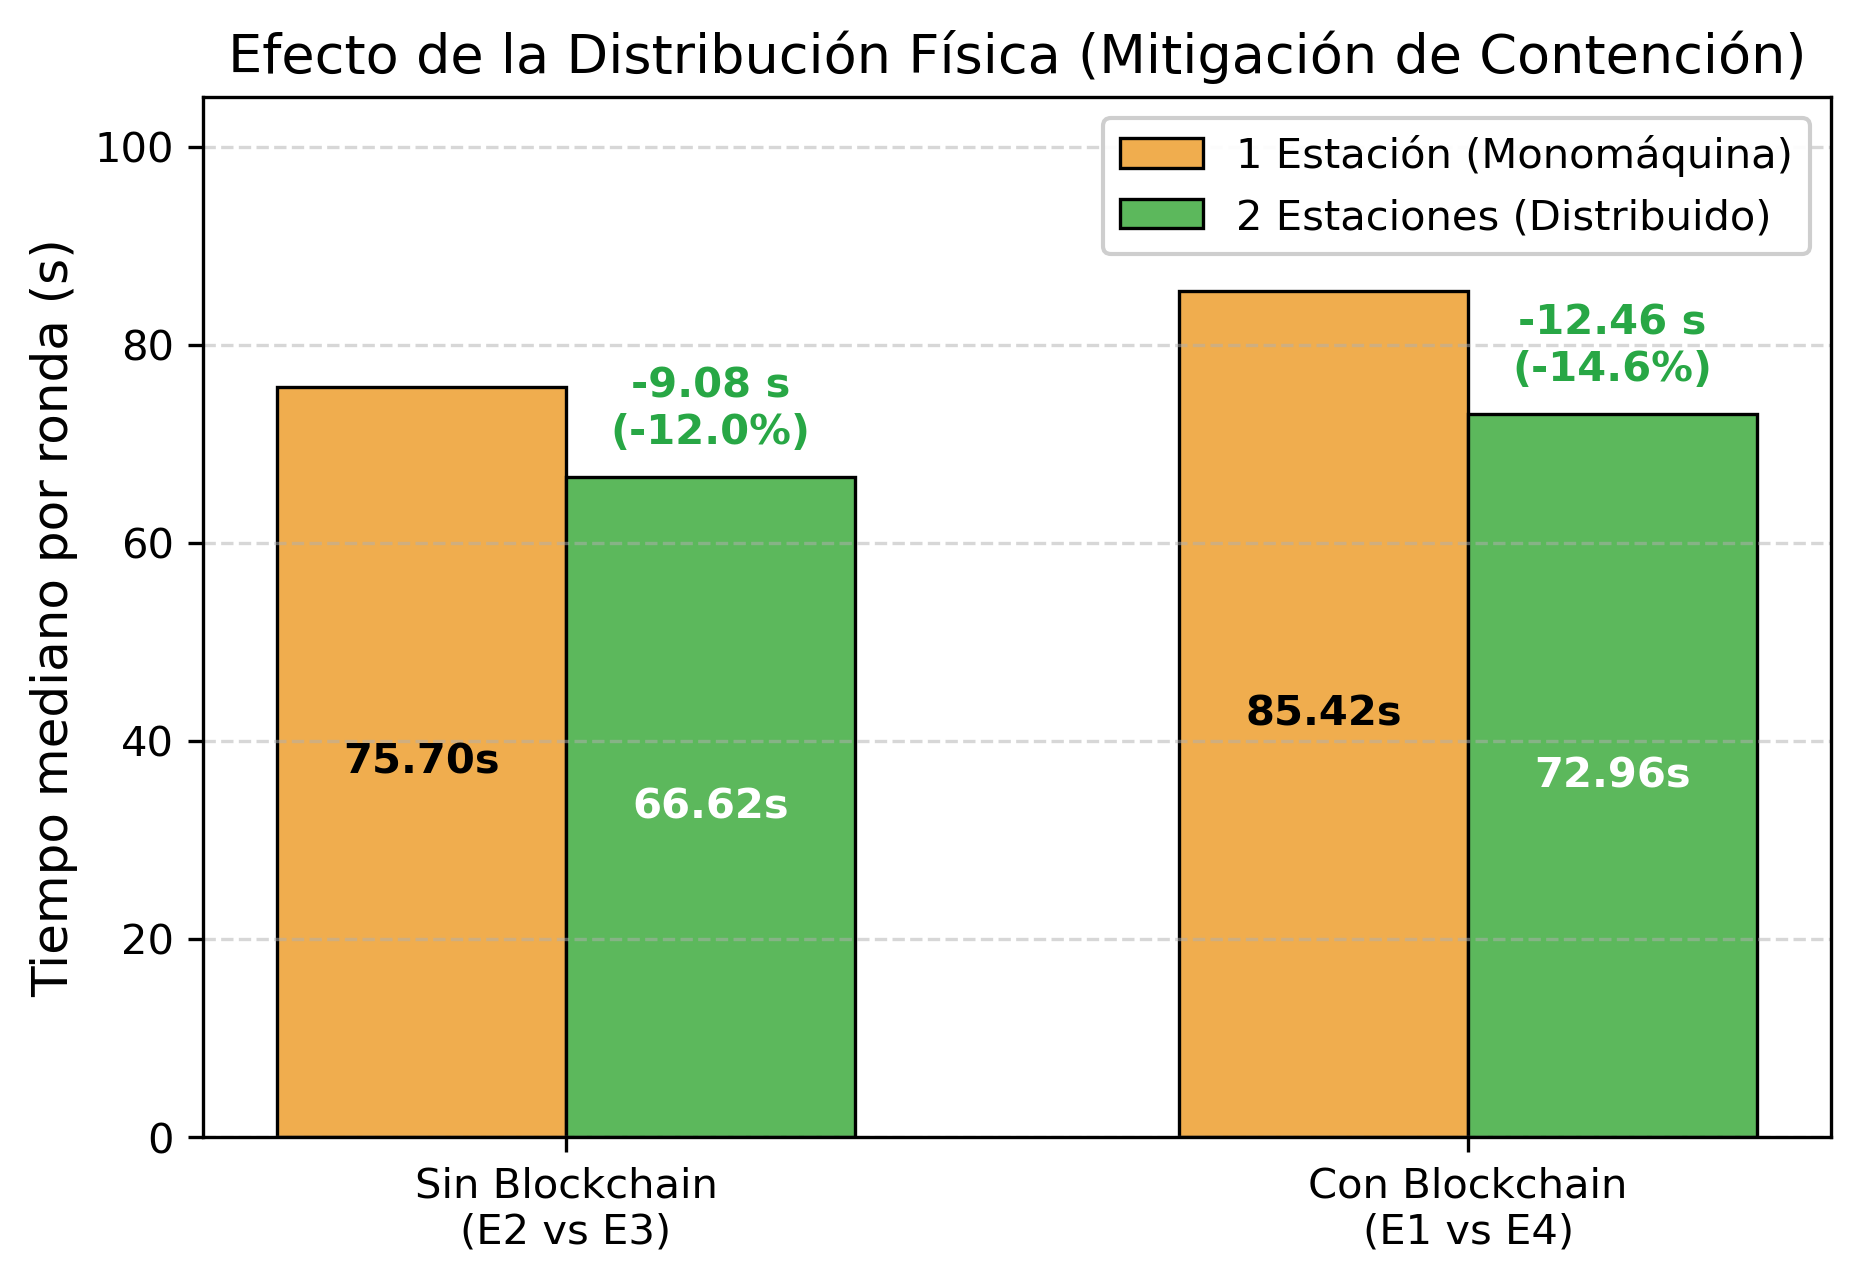
\includegraphics[width=\columnwidth]{figuras/coste_distribucion.png}
    \caption{Efecto de la distribución física de nodos sobre el tiempo de ciclo: mitigación de cuellos de botella de CPU/memoria.}
    \label{fig:coste_dist}
\end{figure}

Para explicar rigurosamente este comportamiento, la Tabla~\ref{tab:desglose_fases} descompone la latencia media de cada fase interna del ciclo federado tanto en los clientes (Estación 2) como en el servidor (Estación 1), evidenciando la correspondencia con las métricas agregadas de la Tabla~\ref{tab:tiempos_resumen}.

\begin{table}[H]
\centering
\caption{Desglose fino de la latencia media por fase en cliente ($T_{\text{client}}$) y servidor ($T_{\text{server}}$) (segundos).}
\label{tab:desglose_fases}
\resizebox{\columnwidth}{!}{%
\begin{tabular}{@{}lcccc|cccc@{}}
\toprule
& \multicolumn{4}{c|}{\textbf{Fases Cliente (Estación 2)}} & \multicolumn{4}{c}{\textbf{Fases Servidor (Estación 1)}} \\
\cmidrule(lr){2-5} \cmidrule(lr){6-9}
\textbf{Exp.} & \textbf{Train} & \textbf{Verif.} & \textbf{IPFS} & \textbf{Tx Besu} & \textbf{Espera} & \textbf{Verif.} & \textbf{FedAvg} & \textbf{Bloque} \\
\midrule
$E_1$ & 94,08 & 0,08 & 0,06 & 2,85 & 98,16 & 0,05 & 0,0065 & 5,14 \\
$E_2$ & 76,45 & 0,00 & 0,00 & 0,00 & 77,02 & 0,00 & 0,0040 & 0,00 \\
\midrule
$E_3$ & 67,62 & 0,00 & 0,00 & 0,00 & 71,07 & 0,00 & 0,0036 & 0,00 \\
$E_4$ & 66,22 & 1,68 & 2,43 & 2,84 & 79,54 & 0,06 & 0,0047 & 2,89 \\
$E_5$ & 65,40 & 1,91 & 3,93 & 2,94 & 82,63 & 0,06 & 0,0079 & 2,99 \\
\bottomrule
\end{tabular}%
}
\end{table}

Los datos de la Tabla~\ref{tab:desglose_fases} confirman tres principios fundamentales:
\begin{enumerate}
    \item \textbf{Desacoplamiento de cómputo:} En las configuraciones distribuidas ($E_3$, $E_4$, $E_5$), el tiempo dedicado exclusivamente a la optimización neuronal con PyTorch se mantiene estrictamente invariante ($\sim 65,4\text{--}67,6$~s), evitando la contención de recursos observada en $E_1$ ($94,08$~s).
    \item \textbf{Sobrecarga de red y verificación acotadas:} La verificación remota vía RPC ($1,68\text{--}1,91$~s en cliente y $\sim 5$~ms en servidor), la transferencia IPFS ($2,43\text{--}3,93$~s) y el cómputo in-memory del multihash de pesos en el servidor ($\sim 52$~ms en el código final, $<0{,}08\%$ del ciclo) añaden una latencia mínima, mientras que el cálculo de FedAvg es despreciable ($< 8$~ms).
    \item \textbf{Correspondencia entre métricas ($T_{\text{client}}$ y $T_{\text{server}}$):} La suma de las cuatro fases locales del cliente (\textit{Train} + \textit{Verif.} + \textit{IPFS} + \textit{Tx Besu}) totaliza con exactitud el tiempo de ciclo reportado en la Tabla~\ref{tab:tiempos_resumen} (por ejemplo, en $E_4$: $66{,}22 + 1{,}68 + 2{,}43 + 2{,}84 = 73{,}17$~s, en plena coherencia con la media de $73{,}29$~s). Paralelamente, la perspectiva del servidor refleja la duración global de la ronda en el agregador ($T_{\text{server}}$), donde el servidor aguarda la concurrencia de todos los clientes (\textit{Espera}, $79{,}54$~s) y añade la confirmación del nuevo modelo consolidado en la cadena (\textit{Bloque}, $2{,}89$~s), totalizando una latencia extremo a extremo de $\approx 82{,}49$~s.
\end{enumerate}

\subsection{Escalado de Consenso Bizantino IBFT 2.0 (4 frente a 7 Validadores)}
En redes permisionadas, la tolerancia a fallos bizantinos sigue el principio $N \ge 3f + 1$, donde $N$ es el conjunto de validadores y $f$ el número máximo de nodos bizantinos o caídos:
\begin{itemize}
    \item Red de 4 validadores ($E_4$): tolera $f=1$ fallo; quórum de firmas necesario $2f+1 = 3$.
    \item Red de 7 validadores ($E_5$): tolera $f=2$ fallos; quórum de firmas necesario $2f+1 = 5$.
\end{itemize}

Al comparar $E_4$ con $E_5$, la mediana por ronda apenas varía de 72,96~s a 73,35~s (+0,39~s), lo que evidencia que la latencia global del ciclo sigue dominada por el entrenamiento local.

\begin{figure}[H]
    \centering
    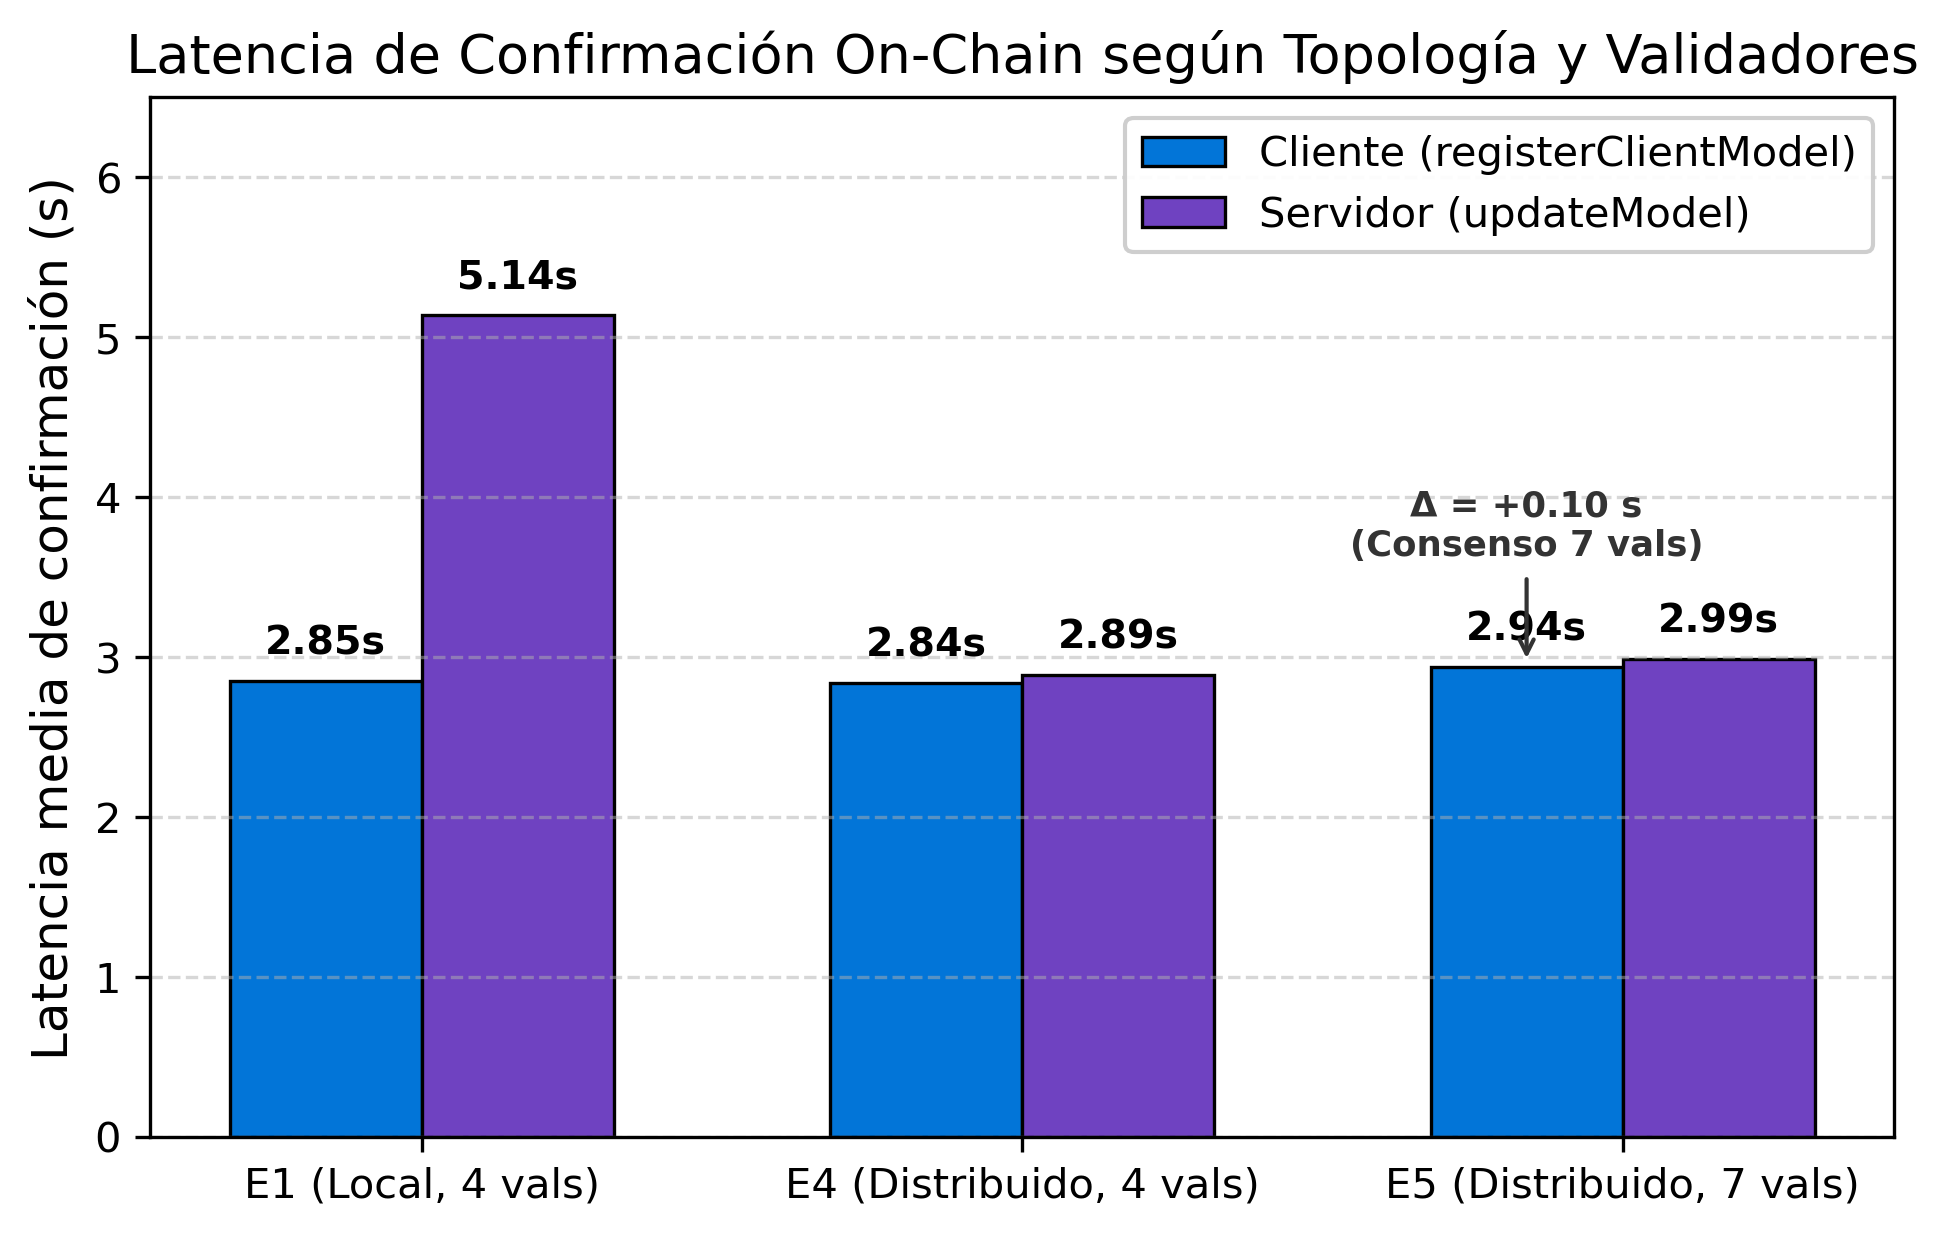
\includegraphics[width=\columnwidth]{figuras/tiempo_confirmacion.png}
    \caption{Tiempo medio de confirmación de transacción según topología y número de validadores en Hyperledger Besu.}
    \label{fig:tiempo_confirmacion}
\end{figure}

Al aislar específicamente el \textbf{tiempo de confirmación de las transacciones on-chain} (Figura~\ref{fig:tiempo_confirmacion}), la complejidad de intercambio de mensajes del algoritmo IBFT~2.0 ($\mathcal{O}(N^2)$ en fases \textit{Prepare} y \textit{Commit}) se manifiesta de manera clara:
\begin{itemize}
    \item Transacción del cliente (\texttt{registerClientModel}): la latencia media pasa de 2,84~s en $E_4$ a 2,94~s en $E_5$ (+0,10~s).
    \item Transacción del servidor (\texttt{updateModel}): la latencia pasa de 2,89~s en $E_4$ a 2,99~s en $E_5$ (+0,10~s).
\end{itemize}
Este incremento simétrico de 100~ms confirma experimentalmente que ampliar la resiliencia bizantina del consorcio de 1 a 2 nodos fallidos no compromete la viabilidad temporal del sistema.

\subsection{Robustez Adversarial y Verificación Experimental de Ataques}
\label{subsec:ataques}
Para validar empíricamente que la arquitectura no solo registra transacciones en condiciones nominales, sino que neutraliza activamente vectores de ataque reales, se implementó una batería de ensayos adversariales controlados en el módulo \texttt{test\_verificacion.py}. El objetivo es evaluar el comportamiento del sistema ante las dos principales amenazas bizantinas en aprendizaje federado no confiable: un servidor central comprometido (ataque descendente) y un nodo participante envenenador (ataque ascendente).

\subsubsection{Prueba 1: Verificación Descendente (Servidor Adulterado frente a Cliente Edge)}
\label{subsubsec:ataque_descendente}
En un entorno federado no confiable, la distribución descendente de parámetros expone a los clientes a dos vectores de riesgo principales: la alteración de los tensores en tránsito por intermediarios de red (\textit{Man-in-the-Middle}) y la bifurcación maliciosa o equivocación del servidor (\textit{server equivocation}), donde un agregador deshonesto intenta distribuir modelos globales distintos o sesgados selectivamente a participantes específicos. Cabe destacar que la validez del modelo global on-chain queda estrictamente acotada a la entidad autorizada gracias al modificador de control de acceso \texttt{onlyServer} en el contrato \texttt{FLRegistry}, el cual revierte cualquier intento de registro por cuentas no autorizadas. Así, la rutina de verificación descendente implementada en el cliente protege de forma autónoma frente a discrepancias entre los pesos recibidos por gRPC y el compromiso sellado institucionalmente en la Blockchain:
\begin{enumerate}
    \item \textbf{Generación y Sellado Oficial:} El servidor legítimo instancia el modelo base \texttt{NetCliente}, serializa los tensores mediante \texttt{pickle.dumps} y los publica en el daemon IPFS local a través del endpoint \texttt{/api/v0/add?pin=false}, obteniendo el CID oficial \texttt{QmQTpgejdzh...}. A continuación, el servidor emite una transacción firmada en la EVM invocando \texttt{updateModel(round, cid\_oficial)} desde su cuenta autorizada (\texttt{0xfe3b55...}), quedando el compromiso criptográfico sellado en el \textbf{Bloque~80}.
    \item \textbf{Inyección Adversarial y Simulación de Discrepancia:} Se emula un escenario adversarial donde se perturban los parámetros transmitidos al cliente inyectando ruido aditivo ($\mathbf{w}_{\text{cand}} = \mathbf{w}_{\text{oficial}} + 0{,}5$) y remitiendo este vector corrupto vía gRPC (simulando alteración en tránsito o un intento del servidor de suministrar una versión discrepante del modelo oficial).
    \item \textbf{Comprobación Cruzada y Aborto Inmediato:} Al recibir la orden de entrenamiento, el cliente edge invoca la función de solo lectura \texttt{getLastModel()} en el Smart Contract mediante una llamada JSON-RPC para recuperar el CID sellado on-chain. Con este identificador descarga de forma paralela el artefacto binario de referencia desde la pasarela IPFS (\texttt{/ipfs/<CID>}) y ejecuta una comparación numérica tensorial elemento a elemento con cota de tolerancia de coma flotante (\texttt{np.allclose(p\_recibido, p\_ipfs, atol=1e-7)}).
\end{enumerate}

\begin{center}
\small
\fbox{
\begin{minipage}{0.95\columnwidth}
\textbf{Algoritmo 1. Verificación Descendente en el Cliente Edge}
\begin{enumerate}
    \item \textbf{Entrada:} Pesos candidatos $\mathbf{w}_{\text{cand}}$ remitidos vía gRPC por el servidor.
    \item Consultar contrato en Besu: $\text{CID}_{\text{onchain}} \leftarrow \texttt{FLRegistry.getLastModel().cid}$
    \item Descargar binario de IPFS: $\mathbf{w}_{\text{ipfs}} \leftarrow \texttt{IPFS.get}(\text{CID}_{\text{onchain}})$
    \item \textbf{Si} $\exists l : \|\mathbf{w}_{\text{cand}, l} - \mathbf{w}_{\text{ipfs}, l}\|_{\infty} > \epsilon$ \textbf{entonces}
    \begin{itemize}
        \item Registrar alerta: \textit{«Discrepancia detectada en pesos recibidos»}
        \item \textbf{ABORTAR} ronda localmente (bloquear backpropagation)
    \end{itemize}
    \item \textbf{Si no:} Aceptar $\mathbf{w}_{\text{cand}}$ y proseguir con el entrenamiento local.
\end{enumerate}
\end{minipage}
}
\end{center}

La Figura~\ref{fig:log_ataque_descendente} ilustra la telemetría real en tiempo de ejecución capturada en la consola del cliente. El proceso íntegro de consulta RPC a Besu, descarga y cotejo tensorial insumió tan solo \textbf{0{,}1486~segundos} (149~ms). Al constatar la discrepancia, el cliente detuvo de forma inmediata la ejecución, impidiendo la contaminación de su modelo local y salvaguardando los datos de entrenamiento privados del vehículo.

\begin{figure}[H]
    \centering
    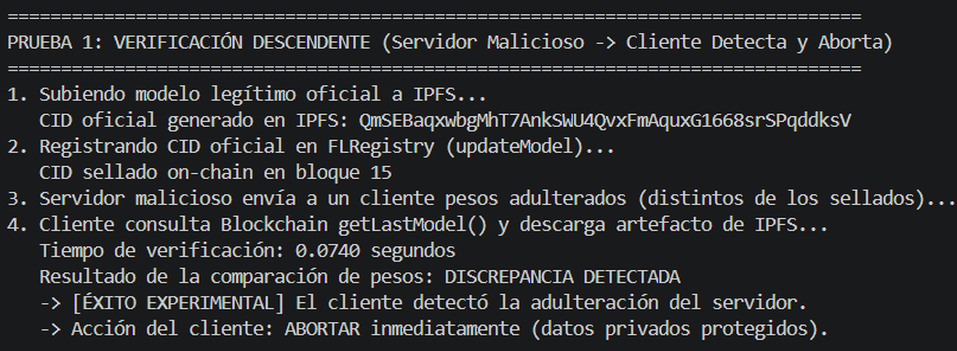
\includegraphics[width=\columnwidth]{figuras/logs_deteccion_ataque_descendent.png}
    \caption{Prueba 1: Registro de consola del nodo cliente detectando la adulteración del modelo frente al CID oficial sellado en el bloque}
    \label{fig:log_ataque_descendente}
\end{figure}

Por su parte, la Figura~\ref{fig:bloque_80_audit} aporta la evidencia inmutable en la cadena de bloques, capturada desde el explorador de la red Hyperledger Besu. En ella se observa el sellado de la transacción \texttt{updateModel} en el \textbf{Bloque~80}, emitida por la dirección del servidor (\texttt{0xfe3b557e...}) con hash criptográfico \texttt{0x973b0b...} y un consumo de gas de 167.460 (límite 500.000). Esta correspondencia unívoca entre el bloque minado y la verificación del cliente valida la consistencia del protocolo.

\begin{figure}[H]
    \centering
    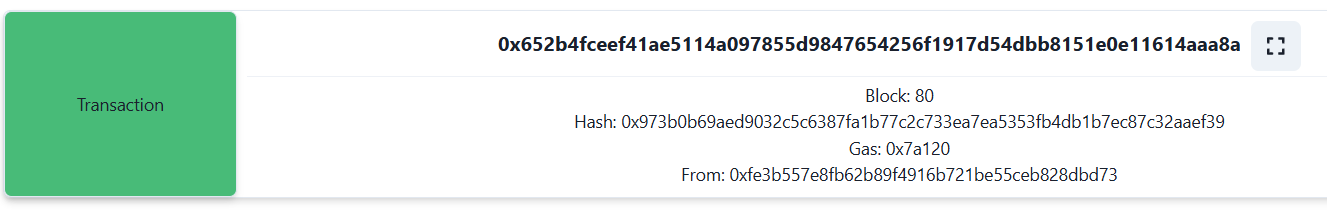
\includegraphics[width=\columnwidth]{figuras/auditoria_grafana_bloque_80.png}
    \caption{Prueba 1: Confirmación en Hyperledger Besu del bloque 80, registrando la transacción oficial \texttt{updateModel} emitida por el servidor agregador.}
    \label{fig:bloque_80_audit}
\end{figure}

\subsubsection{Prueba 2: Verificación Ascendente (Cliente Envenenador frente a Servidor Agregador)}
\label{subsubsec:ataque_ascendente}
La segunda vulnerabilidad crítica consiste en la inyección de gradientes o pesos corruptos por parte de un nodo cliente malicioso (\textit{model poisoning}). Para neutralizarla de raíz, el servidor no se limita a cotejar identificadores, sino que valida de forma cruzada la correspondencia biunívoca entre la carga útil recibida en memoria y el registro inmutable on-chain:
\begin{enumerate}
    \item \textbf{Registro Legítimo On-Chain:} El nodo cliente honesto (cuenta 3, dirección \texttt{0xf17f52...}) publica sus pesos en IPFS y emite una transacción firmada con su clave privada invocando \texttt{registerClientModel}\allowbreak\texttt{(round, cid\_legitimo)}, la cual queda consolidada por los validadores en el \textbf{Bloque~81}.
    \item \textbf{Inyección Adversarial:} Se evalúa el comportamiento ante un intento de inyección donde se remite al servidor una actualización cuyos parámetros o metadatos no coinciden con el compromiso sellado on-chain (emulando tanto el envío de un identificador malicioso \texttt{QmClientFraud...} como el envío de pesos envenenados no correspondientes con el CID registrado).
    \item \textbf{Auditoría Criptográfica y Descarte en FedAvg:} Antes de procesar la agregación matricial de la ronda, el servidor calcula el hash de los tensores recibidos en memoria ($\text{CID}_{\text{calc}}^{(k)}$) y ejecuta una llamada de solo lectura JSON-RPC \texttt{getClientModel(round, address)} sobre el contrato \texttt{FLRegistry} para obtener $\text{CID}_{\text{onchain}}^{(k)}$. Al constatar la discrepancia, la contribución es excluida de forma preventiva.
\end{enumerate}

\begin{center}
\small
\fbox{
\begin{minipage}{0.95\columnwidth}
\textbf{Algoritmo 2. Auditoría Criptográfica y RPC Ascendente en el Servidor Agregador}
\begin{enumerate}
    \item \textbf{Entrada:} Pesos $\mathbf{w}_k^{(t)}$ e identificador $\text{CID}_{\text{rep}}^{(k)}$ reportados por el cliente $k$ con dirección $\text{addr}_k$.
    \item Computar hash de los pesos recibidos: \\
    $\text{CID}_{\text{calc}}^{(k)} \leftarrow \text{Hash}(\mathbf{w}_k^{(t)})$
    \item Consultar registro del cliente en Besu: \\
    $\text{CID}_{\text{onchain}}^{(k)} \leftarrow \texttt{getClientModel}(t, \text{addr}_k)$
    \item \textbf{Si} $\text{CID}_{\text{rep}}^{(k)} \neq \text{CID}_{\text{onchain}}^{(k)}$ \textbf{o} $\text{CID}_{\text{calc}}^{(k)} \neq \text{CID}_{\text{onchain}}^{(k)}$ \textbf{entonces}
    \begin{itemize}
        \item Registrar alerta: \textit{«Discrepancia detectada / Inyección no autenticada»}
        \item \textbf{DESCARTAR} contribución del cliente $k$ del pool de FedAvg
    \end{itemize}
    \item \textbf{Si no:} Incorporar pesos $\mathbf{w}_k^{(t)}$ en la agregación global.
\end{enumerate}
\end{minipage}
}
\end{center}

La Figura~\ref{fig:log_ataque_ascendente} documenta la salida en terminal del servidor agregador. La llamada JSON-RPC a la EVM tomó únicamente \textbf{0{,}0309~segundos} (31~ms). Al constatar que el CID no coincidía con la transacción firmada del cliente, el servidor excluyó al participante de la agregación de forma inmediata, preservando la convergencia y la integridad del modelo global.

\begin{figure}[H]
    \centering
    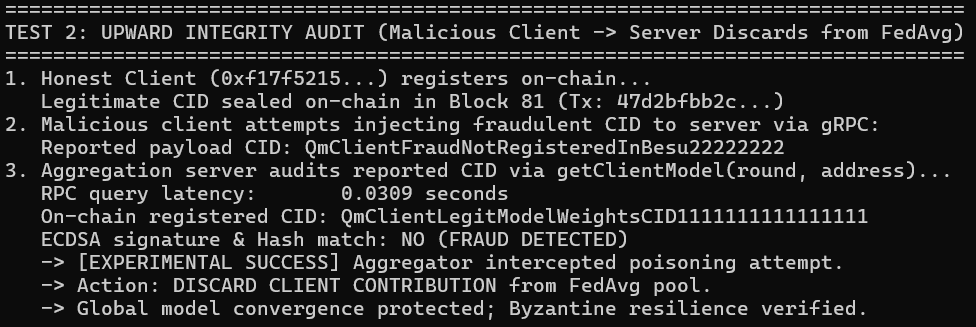
\includegraphics[width=\columnwidth]{figuras/logs_deteccion_ataque_ascendente.png}
    \caption{Prueba 2: Registro de consola del servidor agregador auditando vía RPC el CID del cliente y descartando la contribución fraudulenta}
    \label{fig:log_ataque_ascendente}
\end{figure}

La Figura~\ref{fig:bloque_81_audit} muestra el recibo del \textbf{Bloque~81} en el explorador Besu, donde consta la transacción \texttt{registerClientModel} emitida por la cuenta del cliente (\texttt{0xf17f5215...}) con hash \texttt{0x347899f...} y un consumo de gas de 160.200 (límite 200.000). Dado que el atacante remitió un CID ajeno al sellado en dicho bloque, la verificación cruzada interceptó la inyección adversarial gracias a la resistencia a colisiones de la función hash SHA-256 subyacente al CID de IPFS.

\begin{figure}[H]
    \centering
    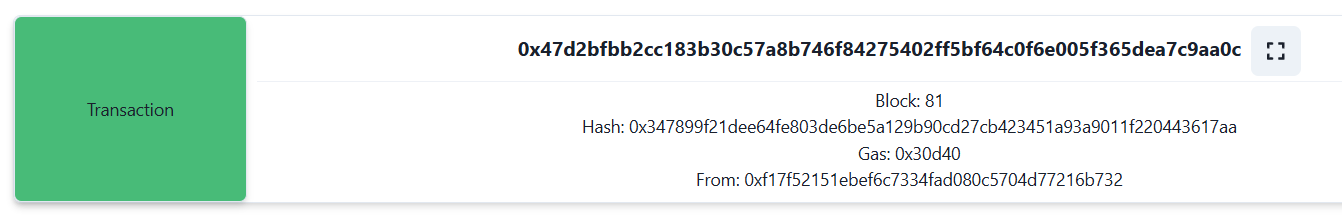
\includegraphics[width=\columnwidth]{figuras/auditoria_grafana_bloque_81.png}
    \caption{Prueba 2: Confirmación forense en Hyperledger Besu del bloque 81, registrando la transacción legítima \texttt{registerClientModel} del nodo cliente.}
    \label{fig:bloque_81_audit}
\end{figure}

\subsubsection{Prueba 3: Auditoría Ex-Post y Verificabilidad Independiente de FedAvg}
\label{subsubsec:auditoria_expost_eval}
Para validar la tercera garantía de integridad formalizada en la Sección~\ref{subsec:auditoria_fedavg}, se evaluó experimentalmente la capacidad de un agente auditor externo o regulador para fiscalizar \textit{a posteriori} y de forma autónoma la fidelidad de la agregación ejecutada por el servidor central. Esta prueba permite auditar matemáticamente si el agregador ha respetado la regla canónica de agregación sin introducir sesgos, omisiones ni alteraciones paramétricas no autorizadas.

El ensayo se ejecutó sobre la Ronda~2 de un entrenamiento real de aprendizaje federado con dos clientes edge concurrentes conectados a la red Hyperledger Besu (contrato \texttt{0x42699A76...}) e IPFS. La Tabla~\ref{tab:trazabilidad_ronda2} sintetiza la cadena de custodia completa de dicha ronda, correlacionando de forma unívoca las cuentas emisoras, las transacciones selladas en los bloques consecutivos 73, 74 y 75, los identificadores multihash IPFS y las latencias registradas.

\begin{table}[H]
\centering
\caption{Cadena de custodia y trazabilidad cruzada on-chain/IPFS durante la Ronda 2 y su fiscalización ex-post.}
\label{tab:trazabilidad_ronda2}
\resizebox{\columnwidth}{!}{%
\begin{tabular}{@{}lcccccc@{}}
\toprule
\textbf{Entidad} & \textbf{Dirección Ethereum} & \textbf{Evento / Método} & \textbf{Bloque Besu} & \textbf{Latencia} & \textbf{CID IPFS} & \textbf{Estado / Resultado} \\
\midrule
Cliente 3 & \texttt{0xf17f5215...} & \texttt{registerClientModel} & Bloque 73 & 0,886 s & \texttt{QmS5ViVf...} & Confirmado on-chain \\
Cliente 2 & \texttt{0x62730609...} & \texttt{registerClientModel} & Bloque 74 & 4,311 s & \texttt{QmNh3TLS...} & Confirmado on-chain \\
Servidor  & \texttt{0xfe3b557e...} & \texttt{updateModel} (FedAvg) & Bloque 75 & 4,709 s & \texttt{QmWF7tJ1...} & Modelo global sellado \\
\midrule
Auditor   & \textit{Externo (Off-chain)} & Reconstrucción FedAvg & Consulta 73--75 & 0,339 s & \texttt{QmWF7tJ1...} & \textbf{$\Delta = 0{,}000000$ (MATCH)} \\
\bottomrule
\end{tabular}%
}
\end{table}

El protocolo de auditoría operó conforme a las siguientes etapas:
\begin{enumerate}
    \item \textbf{Extracción e indexación on-chain:} De forma desacoplada y fuera de banda, el auditor identifica dinámicamente a los clientes participantes $\mathcal{K}_2$ consultando los registros de eventos \texttt{ModelUpdated} de la Ronda~2 en Besu (descubriendo las cuentas del Cliente~2 y Cliente~3) y recupera sus compromisos criptográficos sellados (\texttt{QmNh3TLS...} y \texttt{QmS5ViVf...}), junto con el modelo global reportado por el servidor (\texttt{QmWF7tJ1...}).
    \item \textbf{Descarga y reconstrucción determinista:} El auditor descarga los tres artefactos binarios desde la pasarela IPFS ($2{,}08$~MB por modelo, totalizando $6{,}24$~MB recuperados en $0{,}200$~s acumulados [$0{,}096$~s, $0{,}044$~s y $0{,}060$~s]) y ejecuta la agregación matricial canónica de FedAvg:
    \begin{equation}
    \mathbf{w}_{\text{recon}}^{(2)} = \frac{1}{2}\mathbf{w}_{\text{cli2}}^{(2)} + \frac{1}{2}\mathbf{w}_{\text{cli3}}^{(2)}
    \end{equation}
    generando el hash IPFS del modelo resultante mediante el algoritmo multihash SHA-256.
    \item \textbf{Verificación tensorial y criptográfica:} Se cotejan capa por capa los parámetros del modelo reconstruido frente al modelo global sellado por el servidor en el Bloque~75.
\end{enumerate}

\begin{figure}[H]
    \centering
    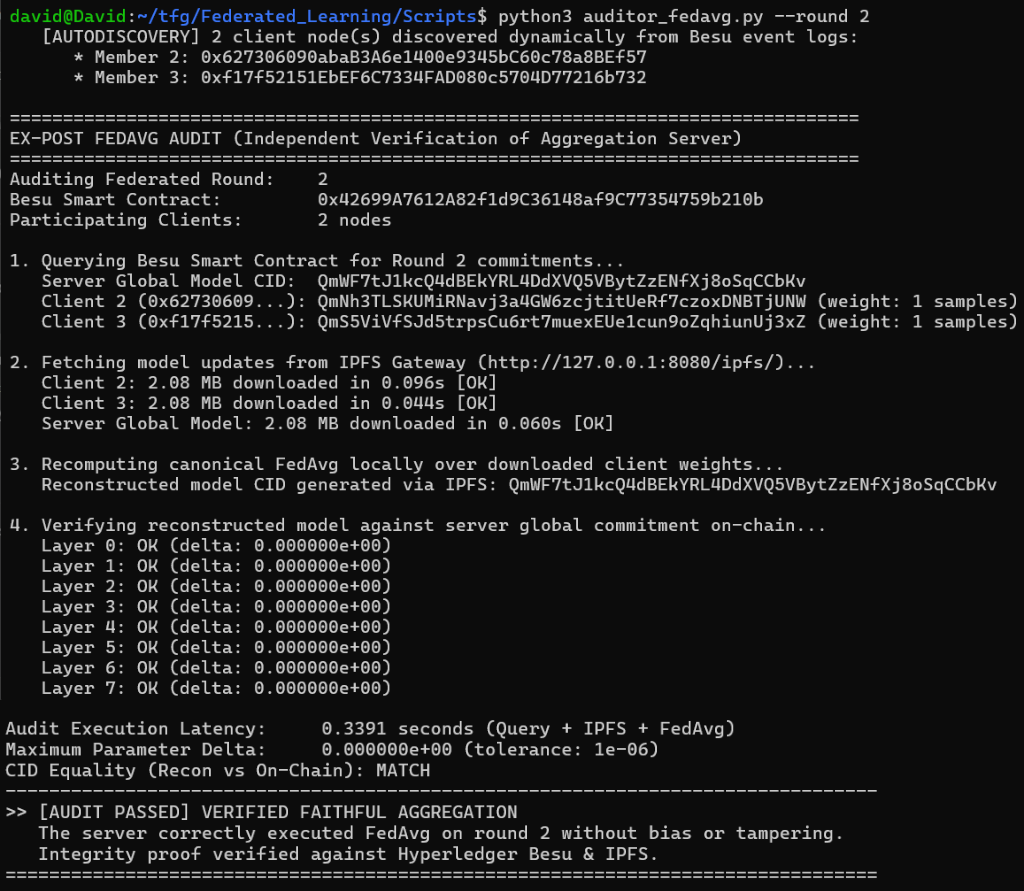
\includegraphics[width=\columnwidth]{figuras/logs_auditoria_expost_fedavg.png}
    \caption{Prueba 3: Registro de consola del auditor independiente reconstruyendo la agregación FedAvg de la Ronda 2 a partir de Besu e IPFS, verificando fidelidad estricta ($\Delta = 0{,}000000$) y coincidencia de CID.}
    \label{fig:log_auditoria_expost}
\end{figure}

\begin{table*}[t]
\centering
\caption{Validación experimental del marco de integridad y auditoría frente a escenarios de manipulación y verificación ex-post.}
\label{tab:resumen_ataques}
\resizebox{\textwidth}{!}{%
\renewcommand{\arraystretch}{1.2}
\begin{tabular}{@{}lcccc@{}}
\toprule
\textbf{Escenario de Prueba} & \textbf{Entidad Defensora / Auditora} & \textbf{Acción Preventiva / Resultado} & \textbf{Latencia} & \textbf{Integridad de Pesos} \\
\midrule
Manipulación en Tránsito / Servidor No Fidedigno & Cliente (Edge) & Intercepción determinista / Aborto preventivo & 0,1486 s & Sin contaminación local \\
Inyección No Autenticada / Cliente No Registrado & Servidor Agregador & Intercepción determinista / Descarte en FedAvg & 0,0309 s & Agregación preservada \\
Auditoría FedAvg Ex-Post & Auditor Independiente & Reconstrucción matemática / Verificación fidedigna & 0,3391 s & Fidelidad exacta ($\Delta = 0$, CID MATCH) \\
\bottomrule
\end{tabular}%
}
\end{table*}

Como refleja la telemetría en tiempo de ejecución capturada en la Figura~\ref{fig:log_auditoria_expost}, la auditoría integral (autodescubrimiento dinámico de participantes vía eventos Besu, consulta RPC de compromisos, descarga de 6,24~MB de IPFS, reconstrucción tensorial y verificación exhaustiva de las 8 capas de la red convolucional) requirió únicamente \textbf{0,3391~segundos}. La discrepancia paramétrica en todas las capas convolucionales y completamente conexas fue estrictamente nula ($\Delta = 0{,}000000\text{e}+00$), derivando en un identificador CID idéntico carácter a carácter al registrado en el Bloque~75 (\texttt{CID Equality: MATCH}), ratificando de forma incontrovertible la concordancia de la agregación.

Asimismo, se evaluó la sensibilidad del mecanismo activando el modo adversarial simulado (\texttt{--simulate-tampering}). Al inyectar una perturbación aditiva deliberada de $+0{,}1$ en los pesos del servidor, el auditor detectó la desviación de forma instantánea en tan solo \textbf{0,1805~segundos} ($\Delta = 1{,}000000\text{e}-01$), registrando una alerta formal de discrepancia no conforme (\texttt{AUDIT FAILED: DISCREPANCY DETECTED}).

\subsubsection{Síntesis de Validación y Alcance de Seguridad}
La Tabla~\ref{tab:resumen_ataques} sintetiza las métricas cuantitativas obtenidas a lo largo de las tres pruebas experimentales de integridad y auditoría.

Estos ensayos constituyen una validación funcional determinista de las primitivas de intercepción criptográfica implementadas en el marco: ante una alteración de los parámetros en tránsito o la ausencia de un compromiso inmutable previamente sellado y firmado en la cadena, el protocolo intercepta la anomalía de manera determinista con tiempos de respuesta en torno a la décima de segundo (149~ms en el cliente, 31~ms en el servidor y $\approx 200$~ms en la auditoría ex-post de FedAvg), impidiendo que los pesos discordantes contaminen los cómputos locales o globales.

Tal como se formalizó en el modelo de amenazas (Sección~\ref{subsec:modelo_amenazas}), conviene remarcar los límites operacionales de este esquema defensivo: la doble verificación en cadena actúa con eficacia contra la adulteración directa de parámetros en tránsito (\textit{tampering}), la emisión no autorizada a nombre de terceros mediante autenticación asimétrica ECDSA y la inyección de modelos disidentes no respaldados on-chain. No obstante, si un nodo malicioso genera una actualización perjudicial mediante manipulación local de sus datos de entrenamiento (\textit{data poisoning} o \textit{label flipping})~\cite{tolpegin2020data} y la firma legítimamente con su clave privada en Besu, el compromiso criptográfico coincidirá formalmente aunque la semántica del modelo esté contaminada. La neutralización de esta tipología de ataques semánticos requiere complementar la trazabilidad con filtros de agregación estadística bizantina (como Krum~\cite{blanchard2017byzantine}, Median o Trimmed-Mean) o mediante la auditoría ex-post de las contribuciones registradas posibilitada por nuestro diseño (Sección~\ref{subsec:auditoria_fedavg}).

\subsection{Consumo y Previsibilidad del Gas en la EVM}
La Figura~\ref{fig:consumo_gas} ilustra el consumo de gas computacional de las operaciones registradas a lo largo de las rondas.

\begin{figure}[H]
    \centering
    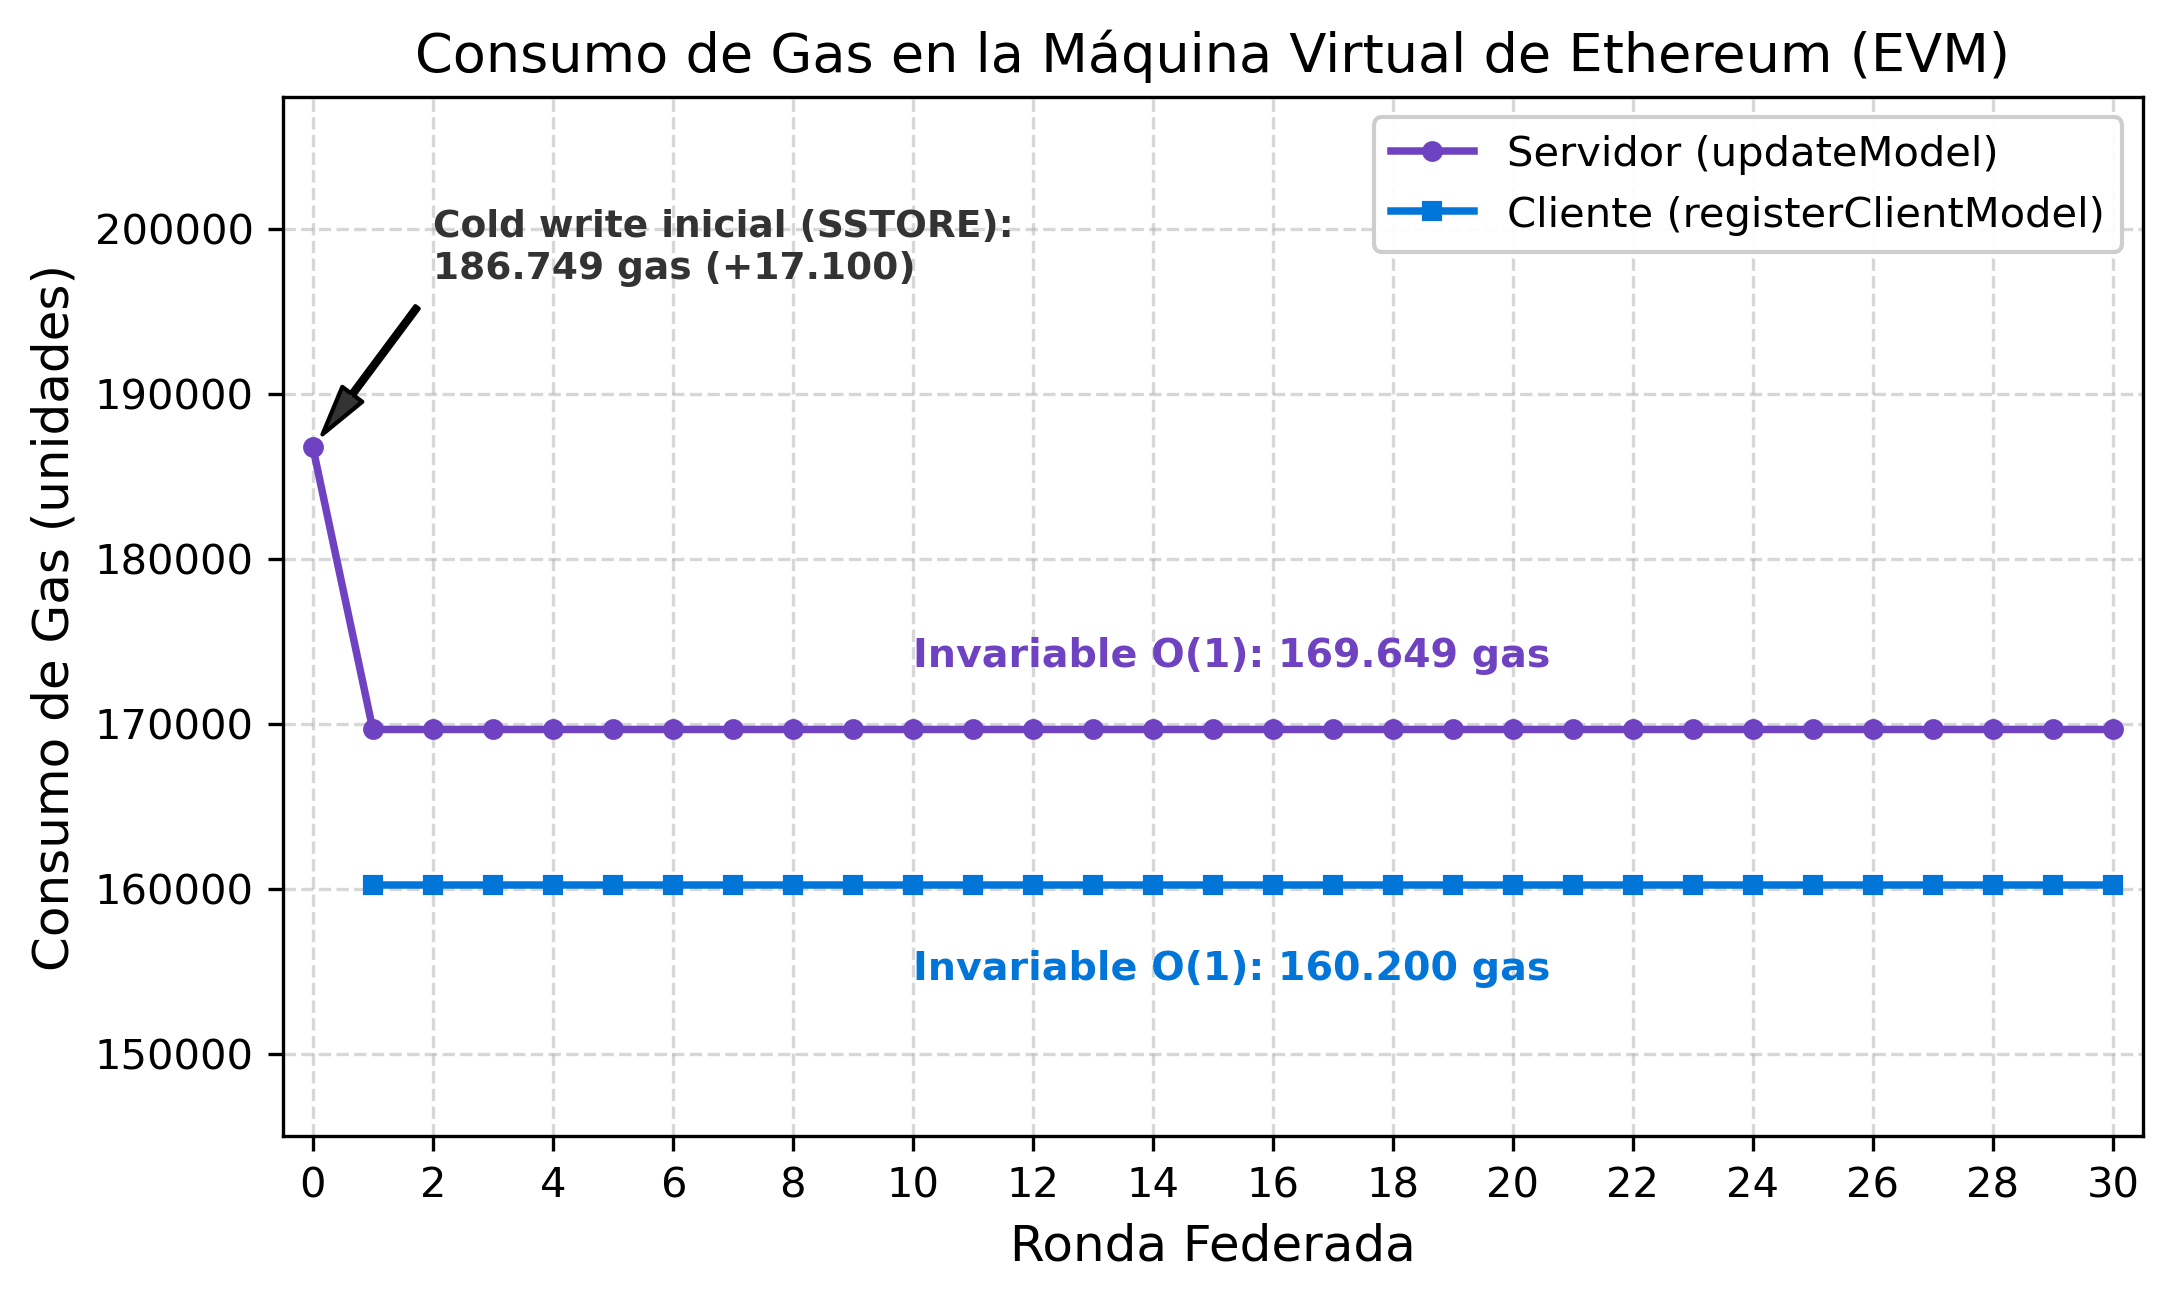
\includegraphics[width=0.70\columnwidth]{figuras/consumo_gas.png}
    \caption{Consumo de gas en la Máquina Virtual de Ethereum por tipo de transacción a lo largo de las 30 rondas.}
    \label{fig:consumo_gas}
\end{figure}

El perfil de consumo resulta rigurosamente constante en todas las iteraciones:
\begin{itemize}
    \item \texttt{registerClientModel}: exactamente \textbf{160.200 unidades de gas}.
    \item \texttt{updateModel}: exactamente \textbf{167.460 unidades de gas}.
\end{itemize}
Conviene destacar que este consumo refleja la versión definitiva del contrato inteligente \texttt{FLRegistry}: la inclusión del modificador de control de acceso \texttt{onlyServer} en \texttt{updateModel} introduce una comprobación de identidad en la EVM (\texttt{SLOAD} y salto condicional sobre \texttt{serverAddress}) que añade únicamente 100 unidades de gas (+0,06\% de sobrecoste respecto a una versión abierta sin control de acceso), manteniendo el coste acotado y plenamente predecible.
La única excepción observable corresponde a la ronda 0 del servidor, que demandó \textbf{184.560 unidades de gas}. Dicha discrepancia (+17.100 unidades) responde al coste de la instrucción \texttt{SSTORE} de la EVM al escribir por primera vez en posiciones de memoria previamente vacías (\textit{cold write}) y modificar el valor del flag booleano \texttt{hasModel}.

La invariabilidad del consumo valida formalmente el diseño desacoplado: al almacenar en el contrato únicamente cadenas de longitud uniforme (los identificadores CIDv0 de IPFS de 46 caracteres que encapsulan el multihash SHA-256 y metadatos acotados), el coste de gas se mantiene estable por transacción e independiente tanto del tamaño del modelo neuronal como del número acumulado de rondas, asegurando un consumo de recursos acotado y predecible en redes de consorcio.

\subsection{Auditoría de Inmutabilidad On-Chain y Trazabilidad Forense}
\label{subsec:auditoria_onchain}
Para verificar empíricamente la correspondencia unívoca entre los eventos del ciclo de vida de Flower y la persistencia inmutable en la cadena de bloques, la Tabla~\ref{tab:auditoria_transacciones} recoge una muestra representativa de los recibos de transacción (\textit{transaction receipts}) extraídos de la telemetría en tiempo de ejecución, correlacionada directamente con la visualización en el explorador de bloques de la red de consorcio (Figura~\ref{fig:auditoria_bloque}).

\begin{table}[H]
\centering
\caption{Muestra de trazabilidad y auditoría forense on-chain.}
\label{tab:auditoria_transacciones}
\resizebox{\columnwidth}{!}{%
\begin{tabular}{@{}cccccc@{}}
\toprule
\textbf{Bloque} & \textbf{Entidad} & \textbf{Evento / Método} & \textbf{Dirección Emisora} & \textbf{Prefijo Tx Hash} & \textbf{Gas EVM} \\
\midrule
8 & Servidor & Despliegue \texttt{FLRegistry} & \texttt{0xfe3b557e...} & \texttt{0x939eb46c...} & 1.999.000 \\
13 & Servidor & \texttt{updateModel} & \texttt{0xfe3b557e...} & \texttt{0xa18e3bb4...} & 167.460 \\
14 & Cliente 2 & \texttt{registerClientModel} & \texttt{0x62730609...} & \texttt{0xc1c7402f...} & 160.200 \\
\midrule
765 & Servidor & \texttt{updateModel} (Ronda 23) & \texttt{0xfe3b557e...} & \texttt{0x4ceabb7a...} & 167.460 \\
783 & Servidor & \texttt{updateModel} (Ronda 24) & \texttt{0xfe3b557e...} & \texttt{0xb9cb75f5...} & 167.460 \\
801 & Servidor & \texttt{updateModel} (Ronda 25) & \texttt{0xfe3b557e...} & \texttt{0xdf69295f...} & 167.460 \\
\bottomrule
\end{tabular}%
}
\end{table}

\begin{figure}[H]
    \centering
    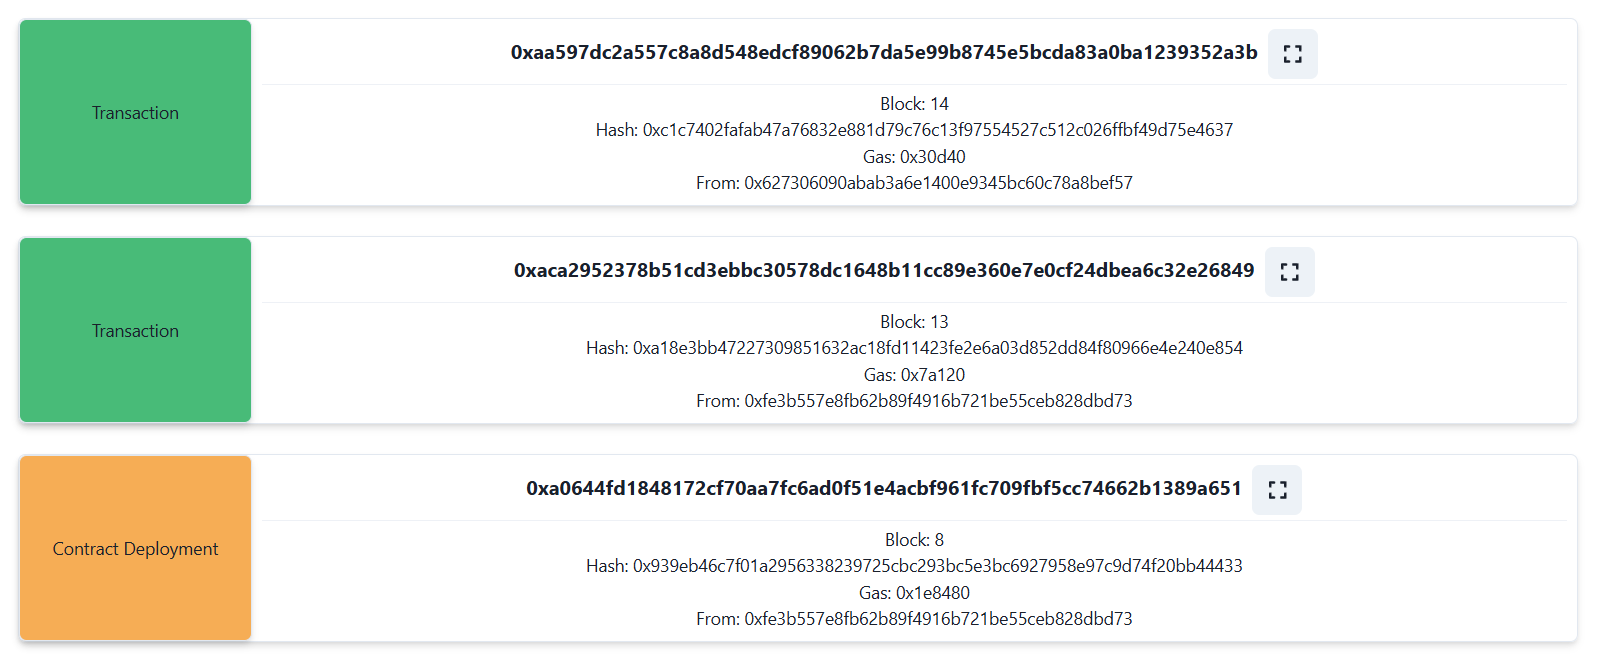
\includegraphics[width=0.96\columnwidth]{figuras/bloque_contrato.png}
    \caption{Auditoría de inmutabilidad on-chain: visualización en el explorador Besu del despliegue del contrato \texttt{FLRegistry} (Bloque~8) por el servidor (\texttt{0xfe3b55...}) junto a transacciones operativas 13 y 14.}
    \label{fig:auditoria_bloque}
\end{figure}

Cada identificador de bloque y hash criptográfico actúa como prueba forense no repudiable, confirmando la viabilidad de la arquitectura para auditorías regulatorias en sistemas vehiculares y de misión crítica.
